%# -*- coding: utf-8-unix -*-
%%==================================================
%% chapter01.tex for SJTU Master Thesis
%%==================================================

%\bibliographystyle{sjtu2}%[此处用于每章都生产参考文献]
\chapter{Introduction}
\label{chap:intro}
\section{Motivation and Contribution}
In many real world applications, data is collected incrementally. For example, the large-scale image classification dataset ImageNet is becoming larger and larger when more notations become available. For another practical example and also the main origination of this project, imagine a commercial system that can classify merchandise correctly based on the image of the merchandise, as illustrated in Fig.~\ref{fig:merchandise}. It has a large potential to be used by automatic robotic arms used in automatic logistics center or autonomous supermarkets. A robotic arm is shown in Fig.~\ref{fig:arm}. Since there will always be new types of merchandise emerging, this system should always adapt to new merchandise types but also not forgetting the learned merchandise types. Thus in this example, the merchandise data is also incremental.

\begin{figure}[!htp]
	\centering
	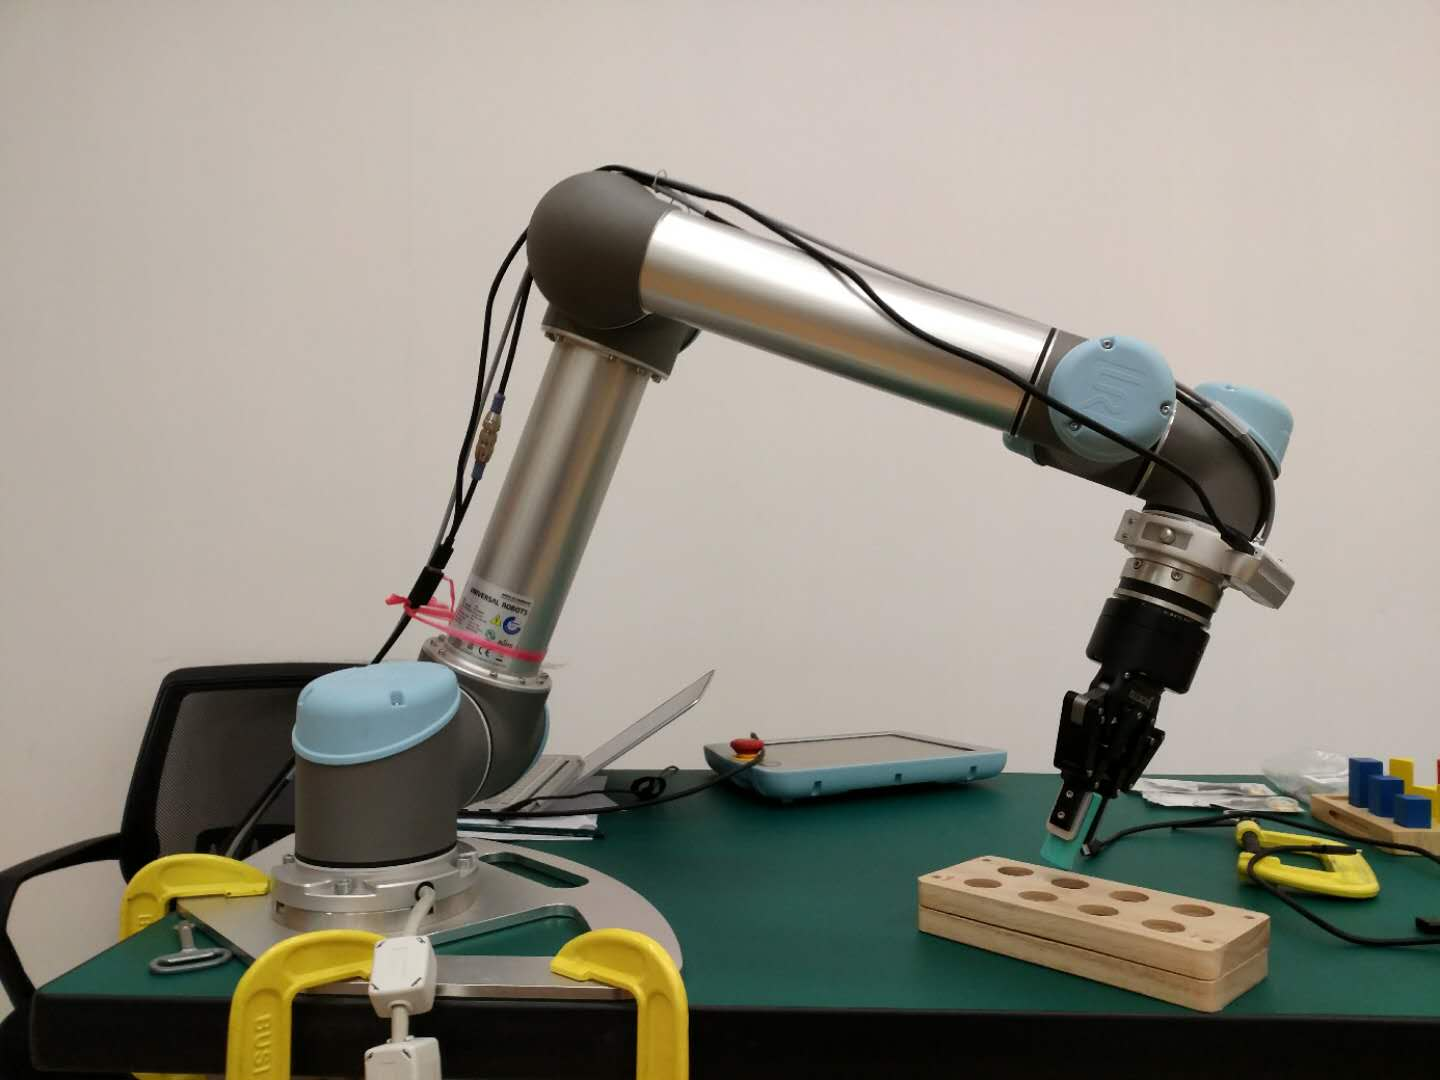
\includegraphics[width=14cm]{arm.jpg}
	\bicaption[Example of a robotic arm for autonomous logistics center]
	{可用于物流系统的机械臂示意图}
	{Example of a robotic arm for autonomous logistics center}
	\label{fig:arm}
\end{figure}
\begin{figure}[!htp]
	\centering
	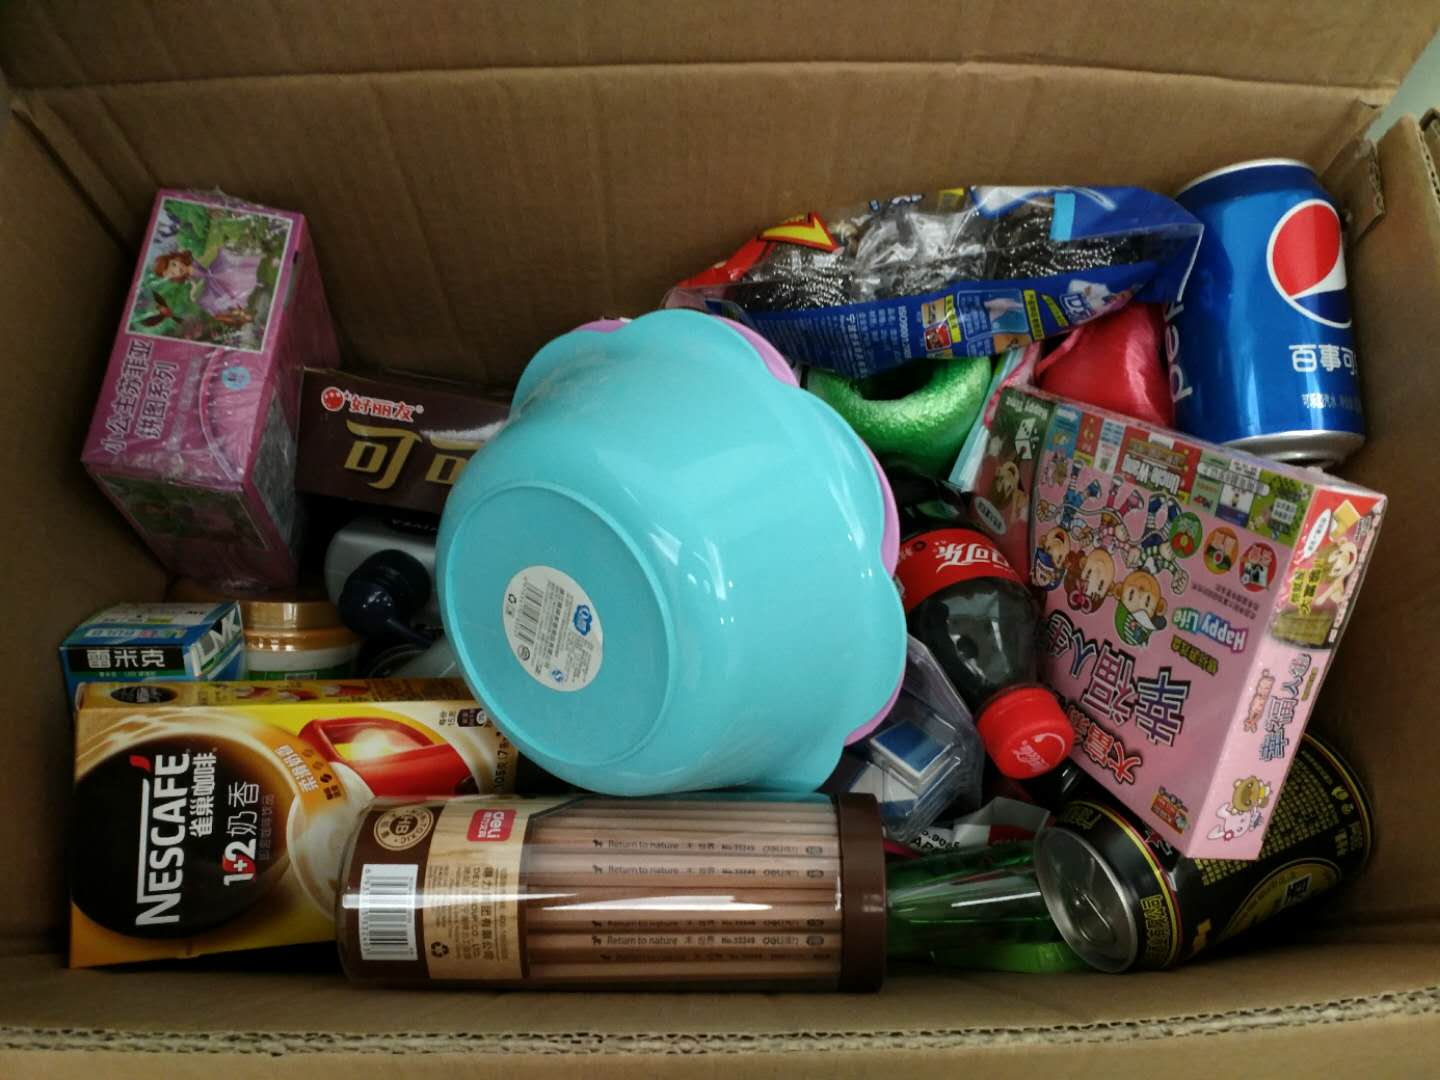
\includegraphics[width=14cm]{merchandise.jpg}
	\bicaption[Example of various types of merchandise]
	{不同类别的商品示意图}
	{Example of various types of merchandise}
	\label{fig:merchandise}
\end{figure}

In recent years, deep learning is the main method to perform classification on these problems. Shown in the examples, it is essential that we had methods that can accommodate the newly increased data quickly based on the previous deep learning model, without having to train the whole model with the entire data from scratch. The reasons are obvious. Training the whole deep learning model from scratch would be too time-consuming and energy-consuming. For example, training a image classification model for ImageNet-1k Dataset\cite{deng2009imagenet} using $32\times4d$ ResNeXt-101\cite{xie2017aggregated} model takes 5 days on 8 GPUS. If we retrain the entire model every time new classes of data or more data from the same class become available, the expense will be enormous. This is even worse in commercial scenarios: imagine several new types of merchandise arrive every day, if we retrain the model from scratch, merchandise would have to wait up to several days to be classified and processed, which is unacceptable for real use.

In this paper, we hope to propose methods to this type of learning problems. It will be smarter to evolve the older model to adapt to newer examples while not forgetting the old ones. A term that describes this kind of problems in literature is called incremental learning. There are many different terms that are relevant to this topic but might be slightly different in the conditions, including lifelong learning, multitask learning, class-incremental learning, etc.\cite{utgoff1989incremental}, which we will discuss in further detail in related work section.

To match closely with real use, we considered class-incremental learning on image classification problems, which means that each time one new class of training data arrive. We conducted our experiments in image classification problems, using the datasets CIFAR-10 and CIFAR-100\cite{krizhevsky2009learning}. We used ResNet\cite{he2016deep} and DenseNet\cite{huang2017densely} as representative deep learning models and showed similar trends, which reveals our method is generic for deep learning models. We proposed and compared between various methods, and showed that we can indeed achieve similar high performance within $5\%$ of the total training time for a model retrain, by using a strong baseline method. Furthermore, we proposed methods that can further trade off between training time and accuracy.

We also noted that incremental learning problem is a fundamental and tough problem and field is relatively premature. There are not many existing works, and our method is still not satisfying for commercial use. We hope more research could be conducted in incremental learning for deep neural networks in the future.
\section{Related work}
\subsection{Deep Learning in Computer Vision}
The first successful use of deep learning comes from image classification area. Since the success of AlexNet\cite{krizhevsky2012imagenet} in 2012, deep learning has developed in a tremendous pace. The performance of image classfication as well as other applications of deep learning improve fast as newer and better model architectures are proposed.

After AlexNet, VGGNet\cite{simonyan2014very} was proposed that used up to more than 30 layers of neural network and significantly improved the performance. At the same time, Google developed a series of deep model architectures\cite{szegedy2015going,szegedy2016inception,szegedy2016rethinking} by utilizing multi-path kernels and outperformed VGGNet. In 2015, Kaiming He proposed ResNet\cite{he2016deep}, using a generic methodology to add shortcut connections between layers that became widely used in later networks. He further refined his work in \cite{he2016identity}, allowing successful training of up to 1202 layers, and surpassed the classification accuracy of human eye. Many variations of ResNet also emerged that year, including Wide ResNet, Later, DenseNet\cite{huang2017densely} proposed to use even denser connections than ResNet, linking every previous layer to the current layer, and replacing sum operator with concatenation. ResNeXt\cite{xie2017aggregated} and Xception\cite{chollet2016xception} make use of group convolution to further improve the performance. In 2017, there continued to have innovations in network architecture which boosted the performance, like Dual Path Networks\cite{chen2017dual} which introduced a novel architecture, and Gradually Updated Neural Networks\cite{qiao2017gradually} that rethinked and improved the calculation method of convolutional layers. Worth mentioning, Google also contributed a lot on automatic searching for the network architecture, and they named the product 'AutoML'. Using their algorithm, they have successfully discovered several interesting and effective architectures, like the state-of-the-art automatically discovered networks NASNet-A\cite{zoph2017learning}, PNASNet\cite{liu2017progressive} and AmoebaNet\cite{real2018regularized}.

Besides the stream of designing better model architectures, some techniques or auxiliary layers are also introduced to boost the network's performance. Dropout\cite{srivastava2014dropout} was proposed to prevent overfitting and improve the performance. It is commonly used in small datasets but is rarely used today on ImageNet dataset. Batch Normalization\cite{ioffe2015batch} enabled much easier training of deep neural networks. By adding batch normalization layer after the convolutional layer, we are able to use much simpler weight initialization and optimization algorithms, and are able to successfully train deeper networks even without residual connections\cite{he2016deep}. Squeeze-and-Excite Block\cite{hu2017squeeze} is a simple but effective component to be placed after each stage of a network. It consists of global pooling and fully connected layers, and re-weights the features from the corresponding stage. It adds really low overhead (very few extra parameters compared to the whole network) but is able to effectively boost the network performance.

To the best of the authors knowledge, the top performing network on the most authoritative image classification dataset ImageNet-1K is SENet-154\cite{hu2017squeeze}, which is mainly composed of a ResNeXt network and Squeeze-and-Excite Blocks. It reaches up to $16.88\%$ top-1 error and $3.58\%$ top-5 error on ImageNet-1K dataset.

\subsection{Incremental Learning}
Traditionally, many papers proposed solutions to this problem based on existing learning models, including decision trees\cite{utgoff1989incremental}, neural networks\cite{polikar2001learn++}, and SVM\cite{diehl2003svm}. In recent years, deep neural networks have enabled much better models with higher accuracy. Accordingly, several relevant papers have proposed solution to incremental learning for deep neural networks. Utilizing the distillation loss proposed by Hinton\cite{hinton2015distilling}, \cite{li2017learning} proposed to use distillation loss in addition to classification loss for new tasks. In this way, past data for the old task can be completely discarded. There are also several papers that evolves the network dynamically when new data/task arrives, like \cite{yoon2017lifelong,rosenfeld2017incremental,sarwar2017incremental,rusu2016progressive}. They carefully design the network transformation such that the output for past data remain the same. ICaRL\cite{rebuffi2017icarl} is a recent proposal for class-incremental systems, that maintain only a limited set of exemplars for old data.

In sum, this is a relatively new area and not much work has been done to make this task perform well.





\parencite{Meta_CN}jfkldsjfklds
\chapter{Background}

\section{Image Classification}
\subsection{Overview}
Image classification problem is one of the core problems in computer vision. The task is to assign every image an label from a predefined set of labels. Although it seems simple, it has a large variety of applications. Many other seemingly different computer vision problems such as segmentation and object detection often take heavy use of the techniques and methods in image classification. 

There are many challenges in this kind of problem, some of which are listed below:
\begin{itemize}
	\item Scale variation. An object in an image may vary by scale.
	\item Viewpoint variation. The viewpoint of the camera might be different, but it should not affect the predictions.
	\item Intra-class variation. The same class often has different appearance, for example red balls and green balls both belong to ball category.
	\item Occlusion. Often many parts of an object is occluded, but we should still be able to recognize it.
\end{itemize}
Therefore, image classification models should ignore the irrelevant variations, but capture the general characteristics to differentiate different categories.

Most common approaches nowadays are data-driven. It means that we can obtain a large amount of training data, and we will be able to test our model on a test set, before real use. The common strategy is to train a model using the annotated training set, i.e., supervised learning, and then compare the accuracy on the test set to measure a model's performance. Concretely, this process can be summarized into the following three steps:
\begin{itemize}
	\item \textbf{Input}: The input is a set of annotated training set, consisting of a set of N images and its corresponding annotated label(the label might not be $100\%$ correct but should be mostly correct for the model to work well.).
	\item \textbf{Learning}: This step is called training a classifier, or learning a model. The task is to use the above mentioned training set to learn to differentiate different classes.
	\item \textbf{Evaluation}: In this step, we evaluate our trained model/classifier on a new set of annotated images that the model has never seen before, and see if the predicted categories match the true labels of the images. 
\end{itemize}

\subsection{Score Function and Loss Function}
In this section, I will introduce linear classification method, the most common basic approach used in recent years that forms the basis of the final layer of deep neural networks. This approach has two major components, a score function that maps the raw image or features to class confidence scores, and a loss function that quantifies the degree to which the confidence scores match the ground truth labels. As shown below, it is in fact an optimization problem with respect to the parameters of the score function.

Let us assume that there is a training set $\mathbf{X}$, consisting of $N$ images $x_i \in R^D$, each annotated with a label of its category $y_i$. Here $i = 1 ...N$ and $y_i \in 1 ... K$. This means that the image dimension is $D$ (for example, $D=32\times32\times3$ for a $32\times32$ pixel colored image) and there are $K$ distinct categories. In linear mapping, we would first apply a linear projection to get the class score $f(x_i; W, b)$:
\begin{align}
f(x_i; W, b) = Wx_i + b
\end{align}

With regards to the loss function, it quantifies the degree to which the class scores match the ground truth labels. Intuitively, the loss function would be low or close to zero if our predictions are very accurate, and it would be very high if the model is doing poorly. Thus, as an optimization problem, we would like to minimize the loss function. We would briefly introduce the SVM loss and softmax loss function here. Note that the softmax loss function is the most commonly used in deep neural networks for image classification.

The Multi-class Support Vector Machine loss is such a loss that it wants the correct class for an image to have a score higher than the other classes by a specified margin $\Delta$,illustrated in Fig.~\ref{fig:svm}. For simplicity, we let $s_i = f(x_i; W, b)$. The multi-class SVM loss can be expressed as:
\begin{align}L_i = \sum_{j\neq y_i} max(0, s_j - s_{y_i} + \Delta)\end{align}
It is also called the hinge loss. The total loss would be the sum of the loss from each class $L_i$.
\begin{figure}[!htp]
	\centering
	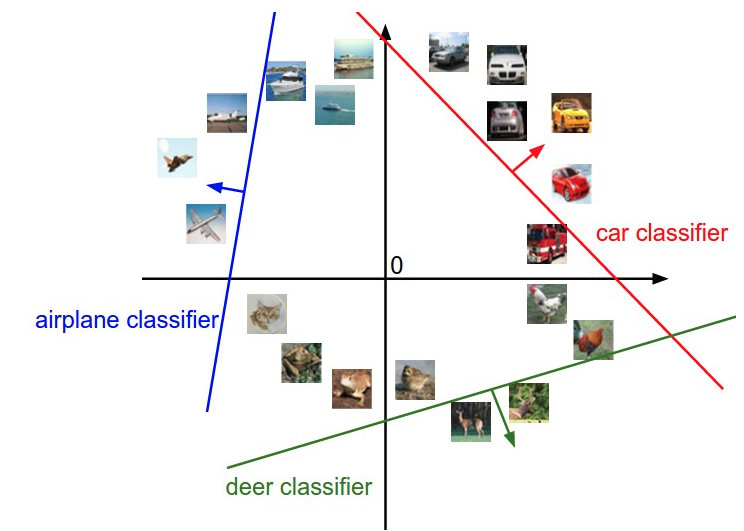
\includegraphics[width=10cm]{svm.png}
	\bicaption[An example of SVM classifier]
	{SVM分类例子例子}
	{An example of SVM classifier}
	\label{fig:svm}
\end{figure}
The softmax loss is a generalization of the binary logistic regression loss to multiple classes. In the softmax loss, we interpret the class scores as the unnormalized log probabilities. Therefore, to obtain the probabilities, we will first exponentiate them and then normalize so that they sum to one: 
\begin{align}
P(Y_i|x_i;W) = \frac{e^{f_{y_i}}}{\sum_j e^{f_j}}
\end{align}, where $f_i = f(x_i; W, b)$.
In this probabilistic interpretation, we then minimize the negative log likelihood of that correct class, which is like performing Maximum Likelihood Estimation. Thus the softmax loss can be written as:
\begin{align}L_i = -log\left( \frac{e^{f_{y_i}}}{\sum_j e^{f_j}}\right)\end{align}
or its equivalent,
\begin{align} L_i = -f_{y_i} + log \sum_j e^{f_j}\end{align}
It is also called the cross-entropy loss. With the linear score function and the loss function, we are ready to extend them to deep neural networks, which will be introduced briefly in the next section.



\section{Deep Neural Networks}
It is often claimed that the area of Neural Networks was originally inspired by biological neural systems. However, the neural network referred in this paper, and including common literature, is a much simplified mathematical operation, compared to real biological neural networks. A basic unit is illustrated in Fig.~\ref{fig:singleneuron}.
\begin{figure}[!htp]
	\centering
	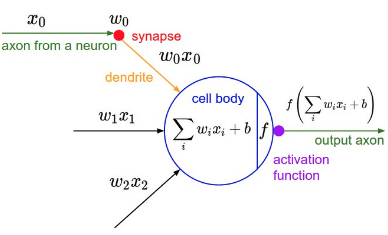
\includegraphics[width=7cm]{singleneuron.png}
	\bicaption[An illustration of a single neuron]
	{单个神经元示意图}
	{An illustration of a single neuron}
	\label{fig:singleneuron}
\end{figure}
Based on the single neuron, we are able to stack many of them to form a multi-layer neural network, as illustrated in Fig.~\ref{fig:nn}.
\begin{figure}[!htp]
	\centering
	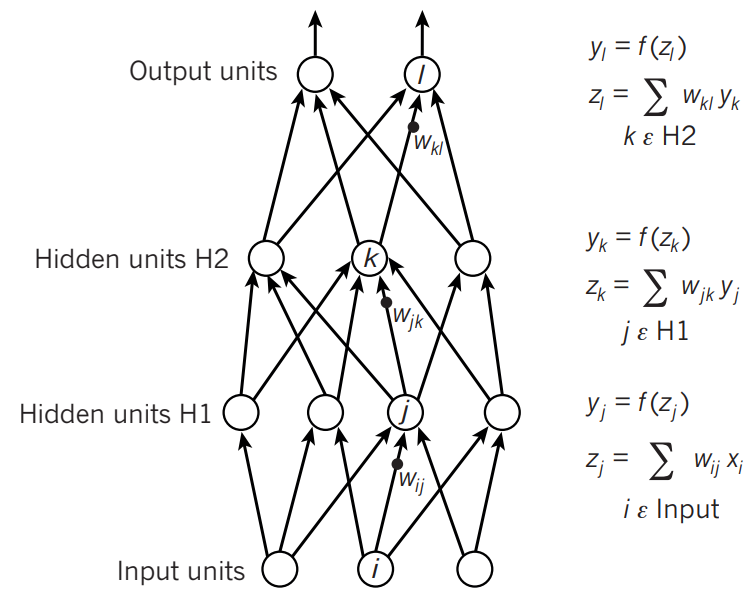
\includegraphics[width=14cm]{nn.png}
	\bicaption[Illustration of Neural Network]
	{多层神经网络示意图}
	{An example of multi-layer neural network. Figure borrowed from \cite{lecun2015deep}}
	\label{fig:nn}
\end{figure}
This paper will be mainly using convolutional neural networks for image recognition. A convolutional layer is different in the mathematical operation, but can feed-forward and back-propagate in the same way. A typical convolutional neural network consists of convolutional layers, pooling layers and fully-connected layers. Fully-connected layer is the same as a single layer neural network. Convolutional layers and pooling layers are illustrated in Fig.~\ref{convolve} and Fig.~\ref{pooling} respectively. 
\begin{figure}[!htp]
	\centering
	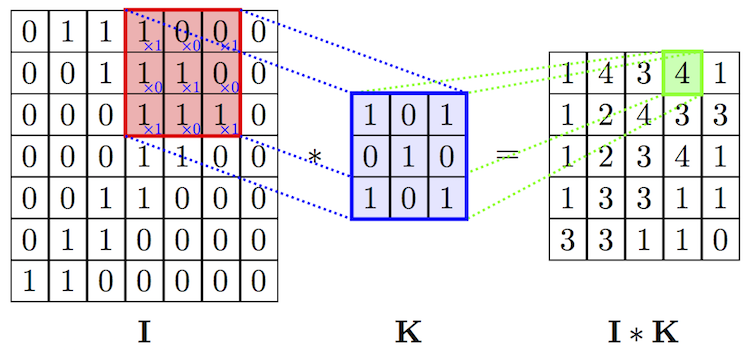
\includegraphics[width=8cm]{convolve.png}
	\bicaption[Illustration of Convolutional Layer]
	{卷积层示意图}
	{Illustration of Convolutional Layer}
	\label{fig:convolve}
\end{figure}
\begin{figure}[!htp]
	\centering
	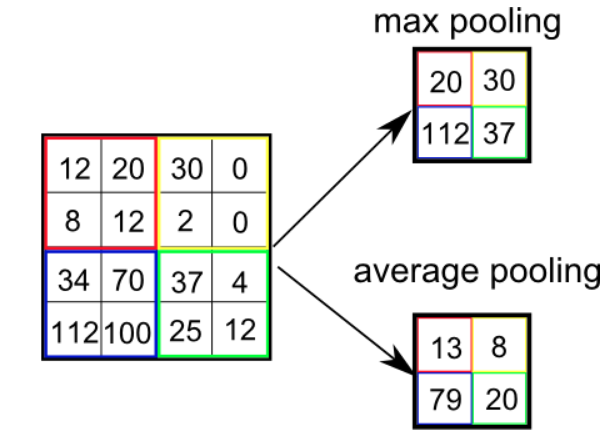
\includegraphics[width=8cm]{pooling.png}
	\bicaption[Illustration of Pooling Layer]
	{池化层示意图}
	{Illustration of Pooling Layer}
	\label{fig:pooling}
\end{figure}

\subsection{Overview}

\subsection{ResNet}
\subsection{DenseNet}
\subsection{ResNeXt}
\section{Hard Negative Mining}


